\chapter{Исследовательская часть}

В данном разделе будет проведен сравнительный анализ времени работы реализаций алгоритмов при различных ситуациях на основе полученных данных.

\section{Технические характеристики}

Технические характеристики устройства, на котором выполнялись замеры времени представлены далее:

\begin{itemize}
	\item операционная система Windows 11 Pro Версия 22H2 (22621.674) \cite{wind};
	\item память 16 ГБ;
	\item процессор 11th Gen Intel(R) Core(TM) i5-11400 2.59 ГГц \cite{proc}.
\end{itemize}

При тестировании компьютер был включен в сеть электропитания. Во время замеров времени выполнения реализаций алгоритмов устройство было нагружено только встроенными приложениями окружения, а также системой тестирования.
\section{Описание проводимых исследований}
Так как в данной работе реализовано несколько алгоритмов вывода трехмерной модели на экран, то можно провести несколько опытов.  
\begin{enumerate}
\item Одной из положительных сторон рейкастинга является возможность параллельного выполнения данного алгоритма. Разные части изображения могут обрабатываться независимо от других. По
этой причине можно обрабатывать части холста одновременно, используя потоки,
таким образом уменьшая общее время работы реализации алгоритма.
Разделение на потоки будет происходить по слеующему принципу: холст разбивается по оси $X$ на равные интервалы, их количество равно количеству логических ядер. В данном эксперементе будет проведено сравнение параллельной версии алгоритма на количестве потоков равному количеству логических ядер ЭВМ, на которой будут проводится замеры времени, и последовательной версии.
\item Во втором эксперементе будет проведено сравнение времени и качества работы реализаций алгоритмов растеризации. Будут сравниваться следующие алгоритмы: использующий интерполяцию, использующий барицентрические координаты, оптимизированные алгоритм использующий барицентрические координаты. Оптимизиция последнего является изменением способа прохода по пикселям --- если в оригинальном алгоритме рассматриваются все пиксели холста, то в текущем они будут рассматриваться змейкой(от границы до границы полигона). 

Все эксперименты будут проведены на кубе, имеющим 12 полигонов.
\end{enumerate}
\section{Использованные средства для замеров времени}
Время работы было замерено с помощью класса \textit{Stopwatch} из библиотеки $System.Diagnostics$ \cite{time}. Перед началом выполнения алгоритма включается таймер методом $Start()$, после выполнения таймер останавливается методом $Stop()$. Для получения времени работы реализаций алгоритмов используется свойство $Elapsed$ того же класса. Возвращаемым значение является структура типа $TimeSpan$, содержащая время работы таймера в часах, минутах, секундах, миллисекундах.

\section{Время выполнения реализаций алгоритмов}
На рисунке \ref{img:graph_sorted}, приведены графические результаты замеров времени работы
алгоритма рейкастинга для параллельного (при количестве потоков, равном количеству
логических ядер ЭВМ, на которой проводились замеры времени, затрачиваемого
реализацией трассировки лучей) и последовательного случаев при разной доле заполнения экрана. На рисунке \ref{img:graph_sorted1}, приведены графические результаты замеров времени работы
алгоритмов растеризации при разной доле заполнения экрана. 


\begin{center}
	\centering{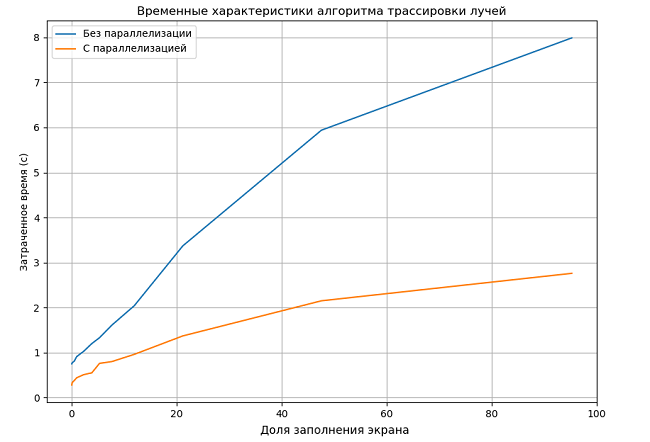
\includegraphics[trim=0 0 0 0cm bb=0 0 484 650]{src/good}}
	\captionof{figure}{Время работы реализаций алгоритма}
	\label{img:graph_sorted}
\end{center}

\begin{center}
	\centering{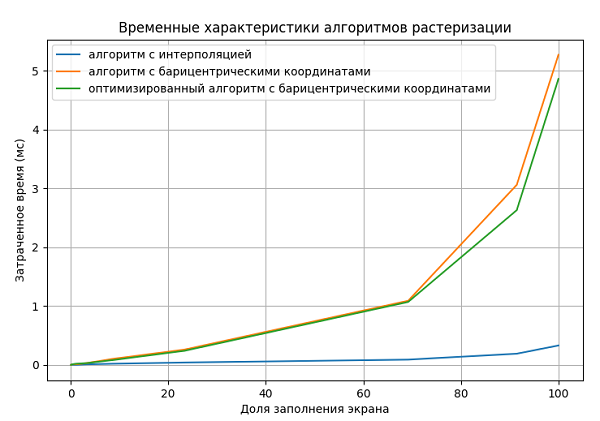
\includegraphics[trim=0 0 0 0cm bb=0 0 600 451]{src/good2}}
	\captionof{figure}{Время работы реализаций алгоритма}
	\label{img:graph_sorted1}
\end{center}
\section{Примеры работы программы}
На рисунках \ref{img:screen} и \ref{img:screen1} приведены прменры работы программы для алгоритмов растеризации использующих интреполяцию и барицентрические координаты соответственно. На экран выводиться лицевая сторона куба.
\begin{center}
	\centering{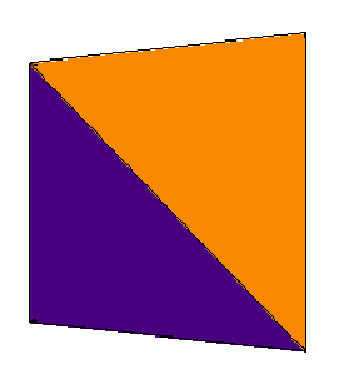
\includegraphics[trim=0 0 0 0cm bb=0 0 400 371]{src/screen_r}}
	\captionof{figure}{Пример работы программы}
	\label{img:screen}
\end{center}
\begin{center}
	\centering{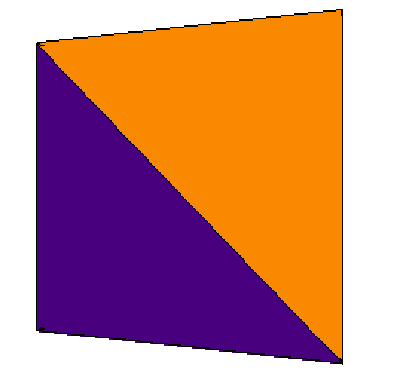
\includegraphics[trim=0 0 0 0cm bb=0 0 400 386]{src/screen_b}}
	\captionof{figure}{Пример работы программы}
	\label{img:screen1}
\end{center}

\section*{Вывод}
\addcontentsline{toc}{section}{Вывод}
Исходя из полученных результатов, трассировка лучей с параллелизацией оказалась быстрее в 2.6 раза на большем заполнении экрана и в 2 раза на меньшем. 

Алгоритмы растеризации использующие баррицентрические координаты оказались значительно медленее при большем заполнении экрана, однако результат выдаваемый ими выглядит лучше с визуальной точки зрения. Так же стоит отметить, что оптимизация алгоритма с барицентрическими координатами не дает особого прироста к скорости выполнения на малой доле заполнения экрана. 
